% Copyright 2006 by Till Tantau
%
% This file may be distributed and/or modified
%
% 1. under the LaTeX Project Public License and/or
% 2. under the GNU Free Documentation License.
%
% See the file doc/generic/pgf/licenses/LICENSE for more details.


% \section{Design Principles}
\section{设计原则}

% This section describes the design principles behind the \tikzname\ frontend, where \tikzname\ means ``\tikzname\ ist \emph{kein} Zeichenprogramm''. To use \tikzname, as a \LaTeX\ user say |\usepackage{tikz}| somewhere in the preamble, as a plain \TeX\ user say |\input tikz.tex|. \tikzname's job is to make your life easier by providing an easy-to-learn and easy-to-use syntax for describing graphics.

本节描述\tikzname 前端背后的设计原则,其中\tikzname\ 表示''\tikzname\ ist \emph{kein} Zeichenprogramm''(\tikzname\ 不是绘图程序)。要使用\tikzname ,作为\LaTeX\ 用户使用 |\usepackage{tikz}|,作为Plain \TeX\ 用户使用 |\input tikz.tex|。\tikzname 的工作是通过提供易于学习和易于使用的图形描述语法来简化您的工作。

% The commands and syntax of \tikzname\ were influenced by several sources. The basic command names and the notion of path operations is taken from \textsc{metafont}, the option mechanism comes from \textsc{pstricks}, the notion of styles is reminiscent of \textsc{svg}, the graph syntax is taken from \textsc{graphviz}. To make it all work together, some compromises were necessary. I also added some ideas of my own, like coordinate transformations.

\tikzname\ 的命令和语法受到多种语法的影响。基本命令名和路径操作的概念来自\textsc{metafont},选项机制来自\textsc{pstricks},样式的概念让人联想到\textsc{svg},图形语法来自\textsc{graphviz}。为了让这一切一起工作,一些妥协是必要的。我还添加了一些自己的想法,比如坐标变换。

% The following basic design principles underlie \tikzname:

以下是基于\tikzname 的基本设计原则:
%
\begin{enumerate}
    % \item Special syntax for specifying points.
    \item 用于指定点的特殊语法。
    % \item Special syntax for path specifications.
    \item 用于指定路径的句法。
    % \item Actions on paths.
    \item 路径上的动作。
    % \item Key--value syntax for graphic parameters.
    \item 图形参数的键值语法。
    % \item Special syntax for nodes.
    \item 用于指定 |node| 的特殊语法。
    % \item Special syntax for trees.
    \item 用于指定 |tree| 的特殊语法。
    % \item Special syntax for graphs.
    \item 用于指定 |graph| 的特殊语法。
    % \item Grouping of graphic parameters.
    \item 图形参数的分组。
    % \item Coordinate transformation system.
    \item 坐标转换系统。
\end{enumerate}


% \subsection{Special Syntax For Specifying Points}
\subsection{用于指定点的特殊语法}

% \tikzname\ provides a special syntax for specifying points and coordinates. In the simplest case, you provide two \TeX\ dimensions, separated by commas, in round brackets as in |(1cm,2pt)|.

\tikzname\ 提供了用于指定点和坐标的特殊语法。在最简单的情况下,提供两个\TeX\ 尺寸,以逗号分隔,用圆括号括起来,如 |(1cm,2pt)|。

% You can also specify a point in polar coordinates by using a colon instead of a comma as in |(30:1cm)|, which means ``1cm in a 30 degrees direction''.

您还可以通过使用冒号而不是使用逗号指定点,像 |(30:1cm)| 这样来指定极坐标中的一个点,这意味着``30度方向上距离原点1cm的点''。

% If you do not provide a unit, as in |(2,1)|, you specify a point in \pgfname's $xy$-coordinate system. By default, the unit $x$-vector goes 1cm to the right and the unit $y$-vector goes 1cm upward.

如果您不提供单位,如在 |(2,1)| 中,您指定\pgfname 的$xy$坐标系中的一个点。默认情况下,单位$x$向量为向右1cm,单位$y$向量为向上1cm。

% By specifying three numbers as in |(1,1,1)| you specify a point in \pgfname's $xyz$-coordinate system.

通过指定 |(1,1,1)| 中的三个数字,您还可以在\pgfname 的$xyz$坐标系统中指定一个点。

% It is also possible to use an anchor of a previously defined shape as in
|(first node.south)|.

也可以使用之前定义的形状的锚点,如 |(first node.south)|。

% You can add two plus signs before a coordinate as in |++(1cm,0pt)|. This means ``1cm to the right of the last point used''. This allows you to easily specify relative movements. For example, |(1,0) ++(1,0) ++(0,1)| specifies the three coordinates |(1,0)|, then |(2,0)|, and |(2,1)|.

可以在坐标前添加两个加号,如 |++(1cm,0pt)|。意思是``最后一个点往右1厘米''。这允许您轻松地指定相对移动。例如 |(1,0) ++(1,0) ++(0,1)| 指定了三个坐标: |(1,0)|,|(2,0)| 和 |(2,1)|。% 

% Finally, instead of two plus signs, you can also add a single one. This also specifies a point in a relative manner, but it does not ``change'' the current point used in subsequent relative commands. For example, |(1,0) +(1,0) +(0,1)| specifies the three coordinates |(1,0)|, then |(2,0)|, and |(1,1)|.

最后,除了两个加号,你还可以使用一个加号。这也以相对的方式指定了一个点,但是它不会``改变''后续相对命令中使用的当前点。例如 |(1,0) +(1,0) +(0,1)| 指定了三个坐标:|(1,0)|,|(2,0)| 和 |(1,1)|。


% \subsection{Special Syntax For Path Specifications}
\subsection{用于指定路径的句法}

% When creating a picture using \tikzname, your main job is the specification of \emph{paths}. A path is a series of straight or curved lines, which need not be connected. \tikzname\ makes it easy to specify paths, partly using the syntax of \textsc{metapost}. For example, to specify a triangular path you use

当使用\tikzname 创建图片时,您的主要任务是指定\emph{路径}。路径是一系列不需要连接的直线或曲线。\tikzname\ 可以很容易地指定路径,部分使用了\textsc{metapost}的语法。例如,为指定三角形路径你需要使用
%
\begin{codeexample}[code only]
(5pt,0pt) -- (0pt,0pt) -- (0pt,5pt) -- cycle
\end{codeexample}
%
% and you get \tikz \draw (5pt,0pt) -- (0pt,0pt) -- (0pt,5pt) -- cycle; when you draw this path.
%
当您绘制此路径时,你会得到 \tikz \draw (5pt,0pt) -- (0pt,0pt) -- (0pt,5pt) -- cycle;。


% \subsection{Actions on Paths}
\subsection{路径上的动作}

% A path is just a series of straight and curved lines, but it is not yet specified what should happen with it. One can \emph{draw} a path, \emph{fill} a path, \emph{shade} it, \emph{clip} it, or do any combination of these. Drawing (also known as \emph{stroking}) can be thought of as taking a pen of a certain thickness and moving it along the path, thereby drawing on the canvas. Filling means that the interior of the path is filled with a uniform color. Obviously, filling makes sense only for \emph{closed} paths and a path is automatically closed prior to filling, if necessary.

路径就是一系列的直线和曲线,还没有制定随着路径命令的执行会发生什么。可以是\emph{绘制}路径,\emph{填充}路径,给它添加\emph{阴影},\emph{剪切}路径,或做这些的任何组合。绘制(也称为\emph{描边})可以被认为是拿一支一定宽度的钢笔,并沿着路径移动,从而在画布上绘画。填充是指路径的内部用统一的颜色填充。显然,填充只对\emph{闭合}路径有意义,如有必要,路径在填充之前会自动关闭。

% Given a path as in |\path (0,0) rectangle (2ex,1ex);|, you can draw it by adding the |draw| option as in |\path[draw] (0,0) rectangle (2ex,1ex);|, which yields \tikz \path[draw] (0,0) rectangle (2ex,1ex);. The |\draw| command is just an abbreviation for |\path[draw]|. To fill a path, use the |fill| option or the |\fill| command, which is an abbreviation for |\path[fill]|. The |\filldraw| command is an abbreviation for |\path[fill,draw]|. Shading is caused by the |shade| option (there are |\shade| and |\shadedraw| abbreviations) and clipping by the |clip| option. There is also a |\clip| command, which does the same as |\path[clip]|, but not commands like |\drawclip|. Use, say, |\draw[clip]| or |\path[draw,clip]| instead.

给定 |\path (0,0) rectangle (2ex,1ex);| 中的路径,您可以通过添加 |draw| 选项来绘制它,如 |\path[draw] (0,0) rectangle (2ex,1ex);|,它会产生 \tikz \path[draw] (0,0) rectangle (2ex,1ex);;|\draw| 命令是 |\path[draw]| 的缩写。要填充一条路径,使用 |fill| 选项或|\fill| 命令,它是 |\path[fill]| 的缩写。|\filldraw| 命令是 |\path[fill,draw]| 的缩写。阴影是由 |shade| 选项(|\shade| 和 |\shadedraw| 缩写)以及剪切是由 |clip| 选项完成的。还有一个 |\clip| 命令,它的作用与 |\path[clip]| 相同,但不是像 |\drawclip| 这样的命令,一般来说,使用 |\draw[clip]| 或 |\path[draw,clip]| 代替它。

% All of these commands can only be used inside |{tikzpicture}| environments.

所有这些命令只能在 |{tikzpicture}| 环境中使用。

% \tikzname\ allows you to use different colors for filling and stroking.

\tikzname\ 允许您使用不同的颜色进行填充和描边。


% \subsection{Key--Value Syntax for Graphic Parameters}
\subsection{图形参数的键值语法}

% Whenever \tikzname\ draws or fills a path, a large number of graphic parameters influences the rendering. Examples include the colors used, the dashing pattern, the clipping area, the line width, and many others. In \tikzname, all these options are specified as lists of so called key--value pairs, as in |color=red|, that are passed as optional parameters to the path drawing and filling commands. This usage is similar to \textsc{pstricks}. For example, the following will draw a thick, red triangle;

每当\tikzname\ 绘制或填充路径时,大量图形参数都会影响呈现效果。包括所使用的颜色、点划模式、剪切区域、线宽以及其他许多内容。在\tikzname 中,所有这些选项都指定为所谓的键值对列表,如 |color=red| 中所示,它们作为可选参数传递给路径绘制和填充命令。这种用法类似于\textsc{pstricks}。例如,下面会画一个红色的粗三角形;
%
\begin{codeexample}[]
\tikz \draw[line width=2pt,color=red] (1,0) -- (0,0) -- (0,1) -- cycle;
\end{codeexample}


% \subsection{Special Syntax for Specifying Nodes}
\subsection{用于指定 \texttt{node} 的特殊语法}

% \tikzname\ introduces a special syntax for adding text or, more generally, nodes to a graphic. When you specify a path, add nodes as in the following example:

\tikzname\ 引入了一种特殊语法,用于向图形添加文本,或者更一般地,添加节点。在指定路径时,添加节点,如下例所示:
%
\begin{codeexample}[]
\tikz \draw (1,1) node {text} -- (2,2);
\end{codeexample}
%
% Nodes are inserted at the current position of the path, but either \emph{after} (the default) or \emph{before} the complete path is rendered. When special options are given, as in |\draw (1,1) node[circle,draw] {text};|, the text is not just put at the current position. Rather, it is surrounded by a circle and this circle is ``drawn''.
%
节点插入到路径的当前位置,但是要么在完整路径绘制\emph{之后}(默认)呈现,要么在完整路径绘制\emph{之前}呈现。当给出特殊选项时,如 |\draw (1,1) node[circle,draw] {text};|,文本不只是放在当前位置。相反,它被一个圆圈包围着,这个圆圈被``绘制''出来。

% You can add a name to a node for later reference either by using the option |name=|\meta{node name} or by stating the node name in parentheses outside the text as in |node[circle](name){text}|.

您可以通过使用选项 |name=|\meta{节点名} 或在文本外的括号中声明节点名称,如 |node[circle](节点名) {text}| 中所示,向节点添加名称以供以后引用。

% Predefined shapes include |rectangle|, |circle|, and |ellipse|, but it is possible (though a bit challenging) to define new shapes.

预定义的形状包括 |rectangle|、|circle| 和 |ellipse|,但也可以定义新形状(尽管这有些挑战性)。


% \subsection{Special Syntax for Specifying Trees}
\subsection{用于指定 \texttt{tree} 的特殊语法}

% The ``node syntax'' can also be used to draw tress: A |node| can be followed by any number of children, each introduced by the keyword |child|. The children are nodes themselves, each of which may have children in turn.

``节点语法''也可以用来绘制树状结构:一个 |node| 后面可以跟着任意数量的子节点,每个子节点都由关键字 |child| 引入。子节点本身是节点,每个节点可以依次有子节点。
%
\begin{codeexample}[]
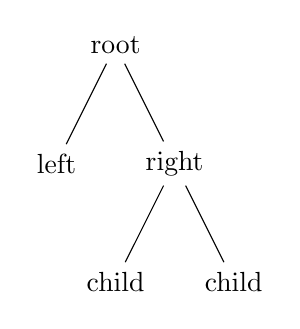
\begin{tikzpicture}
  \node {root}
    child {node {left}}
    child {node {right}
      child {node {child}}
      child {node {child}}
    };
\end{tikzpicture}
\end{codeexample}
%
% Since trees are made up from nodes, it is possible to use options to modify the way trees are drawn. Here are two examples of the above tree, redrawn with different options:
%
由于树是由节点组成的,所以可以使用选项来修改树的绘制方式。下面是上述树的两个例子,用不同的选项重新绘制:
%
\begin{codeexample}[preamble={\usetikzlibrary{arrows.meta,trees}}]
\begin{tikzpicture}
  [edge from parent fork down, sibling distance=15mm, level distance=15mm,
   every node/.style={fill=red!30,rounded corners},
   edge from parent/.style={red,-{Circle[open]},thick,draw}]
  \node {root}
      child {node {left}}
      child {node {right}
        child {node {child}}
        child {node {child}}
      };
\end{tikzpicture}
\end{codeexample}

\begin{codeexample}[]
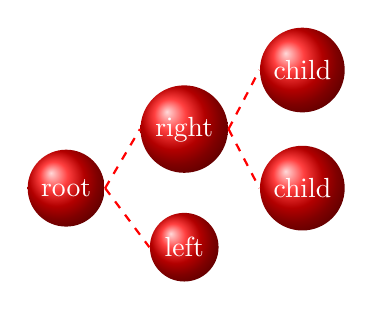
\begin{tikzpicture}
  [parent anchor=east,child anchor=west,grow=east,
   sibling distance=15mm, level distance=15mm,
   every node/.style={ball color=red,circle,text=white},
   edge from parent/.style={draw,dashed,thick,red}]
  \node {root}
      child {node {left}}
      child {node {right}
        child {node {child}}
        child {node {child}}
      };
\end{tikzpicture}
\end{codeexample}


% \subsection{Special Syntax for Graphs}
\subsection{用于指定 \texttt{graph} 的特殊语法}

% The |\node| command gives you fine control over where nodes should be placed, what text they should use, and what they should look like. However, when you draw a graph, you typically need to create numerous fairly similar nodes that only differ with respect to the name they show. In these cases, the |graph| syntax can be used, which is another syntax layer build ``on top'' of the node syntax.

|\node| 命令可以很好地控制节点应该放置在何处、节点应该使用什么文本以及节点的外观。但是,在绘制图形时,通常需要创建许多非常类似的节点,这些节点的不同之处在于它们所显示的名称。在这些情况下,可以使用 |graph| 语法,这是在节点语法之上构建的另一个语法层。
%
\begin{codeexample}[preamble={\usetikzlibrary{graphs}}]
\tikz \graph [grow down, branch right] {
  root -> { left, right -> {child, child} }
};
\end{codeexample}
%
% The syntax of the |graph| command extends the so-called \textsc{dot}-notation used in the popular \textsc{graphviz} program.
%
|\graph| 命令的语法扩展了流行的\textsc{graphviz}程序中使用的所谓的\textsc{dot}表示法。

% Depending on the version of \TeX\ you use (it must allow you to call Lua code, which is the case for Lua\TeX), you can also ask \tikzname\ to do automatically compute good positions for the nodes of a graph using one of several integrated \emph{graph drawing algorithms}.

根据您使用的\TeX\ 的版本(它必须允许您调用Lua代码,这是Lua\TeX 的情况),您还可以要求\tikzname\ 使用几种集成的\emph{图形绘制算法}之一来自动计算图形节点的良好位置。


% \subsection{Grouping of Graphic Parameters}
\subsection{图形参数的分组}

% Graphic parameters should often apply to several path drawing or filling commands. For example, we may wish to draw numerous lines all with the same line width of 1pt. For this, we put these commands in a |{scope}| environment that takes the desired graphic options as an optional parameter. Naturally, the specified graphic parameters apply only to the drawing and filling commands inside the environment. Furthermore, nested |{scope}| environments or individual drawing commands can override the graphic parameters of outer |{scope}| environments. In the following example, three red lines, two green lines, and one blue line are drawn:

图形参数应该经常应用于几个路径绘制或填充命令。例如,我们可能希望绘制多条线,所有线宽都为1pt。为此,我们将这些命令放在 |{scope}| 环境中,该环境将所需的图形选项作为可选参数。当然,指定的图形参数仅应用于环境中的绘图和填充命令。此外,嵌套 |{scope}| 环境或单个绘制命令可以覆盖外部 |{scope}| 环境的图形参数。在下面的例子中,画了三条红线,两条绿线,一条蓝线:
%
\begin{codeexample}[]
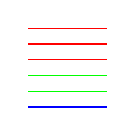
\begin{tikzpicture}
  \begin{scope}[color=red]
    \draw (0mm,10mm) -- (10mm,10mm);
    \draw (0mm, 8mm) -- (10mm, 8mm);
    \draw (0mm, 6mm) -- (10mm, 6mm);
  \end{scope}
  \begin{scope}[color=green]
    \draw             (0mm, 4mm) -- (10mm, 4mm);
    \draw             (0mm, 2mm) -- (10mm, 2mm);
    \draw[color=blue] (0mm, 0mm) -- (10mm, 0mm);
  \end{scope}
\end{tikzpicture}
\end{codeexample}

% The |{tikzpicture}| environment itself also behaves like a |{scope}| environment, that is, you can specify graphic parameters using an optional argument. These optional apply to all commands in the picture.

|{tikzpicture}| 环境本身的行为也类似于 |{scope}| 环境,也就是说,您可以使用可选参数指定图形参数。这些可选命令适用于图片中的所有命令。


% \subsection{Coordinate Transformation System}
\subsection{坐标转换系统}

% \tikzname\ supports both \pgfname's \emph{coordinate} transformation system to perform transformations as well as \emph{canvas} transformations, a more low-level transformation system. (For details on the difference between coordinate transformations and canvas transformations see Section~\ref{section-design-transformations}.)

\tikzname\ 同时支持\pgfname 的\emph{坐标}转换系统来执行转换,以及\emph{画布}转换,这是一种更低级的转换系统。(关于坐标转换和画布转换之间区别的详细信息,请参阅第\ref{section-design-transformations}节。)

% The syntax is set up in such a way that it is harder to use canvas transformations than coordinate transformations. There are two reasons for this: First, the canvas transformation must be used with great care and often results in ``bad'' graphics with changing line width and text in wrong sizes. Second, \pgfname\ loses track of where nodes and shapes are positioned when canvas transformations are used. So, in almost all circumstances, you should use coordinate transformations rather than canvas transformations.

语法的设置使得使用画布转换比使用坐标转换更困难。这样做有两个原因:首先,画布转换的使用必须非常小心,经常会导致``糟糕''的图形,改变了线宽和文本的大小。其次,当使用画布转换时,\pgfname\ 失去了对节点和形状位置的跟踪。因此,在几乎所有的情况下,您应该使用坐标转换而不是画布转换。

